\chapter{Eksperymenty}

W niniejszym rozdziale przedstawiony został krótki opis środowiska testowego oraz przebieg testów układu do zmiany przełożeń.

\section{Środowisko testowe}
Wszystkie eksperymenty przeprowadzone zostały w sposób stacjonarny. Zamontowanie roweru na dedykowanym stojaku umożliwia swobodną symulację dowolnych scenariuszy testowych. Akwizcyja danych sterownika układu jest w takim przypadku zdecydowanie mniej problematyczna, ponieważ nie jest konieczne stosowanie protokołów transmisji bezprzewdowej. 
Na potrzeby testów, wykonana została aplikacja przedstawiająca, w formie przebiegów czasowych, kluczowe parametry układu. Wykorzystano język C++ oraz zestaw bibliotek Qt. Komunikacja pomiędzy sterownikiem a aplikacją nawiązana została za pomocą intefrejsu szeregowego UART(ang. \textit{Universal Asynchronous Receiver and Transmitter}). Sterownik pracujący w trybie testowania, wysyła zastaw danych do komputera PC z częstotliwością 20Hz. Zestaw danych, składa się z chwilowych wartości:
\begin{itemize}
 \item
 kąta nachylenia podłoża,
 \item
 kadencji,
 \item
 prędkości liniowej roweru,
 \item
 wybranego biegu,
 \item
 stanu przycisku redukującego przełożenie,
 \item
 stanu przycisku zwiększającego przełożenie,
 \item
 trybu pracy sterownia.
 \end{itemize}
 
Slot czasowy dla danych prezentowanych na przebiegach jest stały i wynosi 16 sekund. We wszystkich trybach automatycznych przedstawione są również przyjęte zakresy kadencji, a w trybie sportowym dodatkowo zakres kąta nachylenia podłoża.
 
\section{Wyniki tesów}

Poniżej zaprezentowano wyniki testów wybranych scenariuszy, potwierdzające zgodność działania sterownika układu z założeniami, przedstawionymi w pkt. \textcolor{red}{pktFinalny}
\subsection{Tryb ręczny}
Podstawowa funkcjonalność układu to zmiana przełożeń w trybie ręcznym. 
\begin{figure}[h]
    \centering
    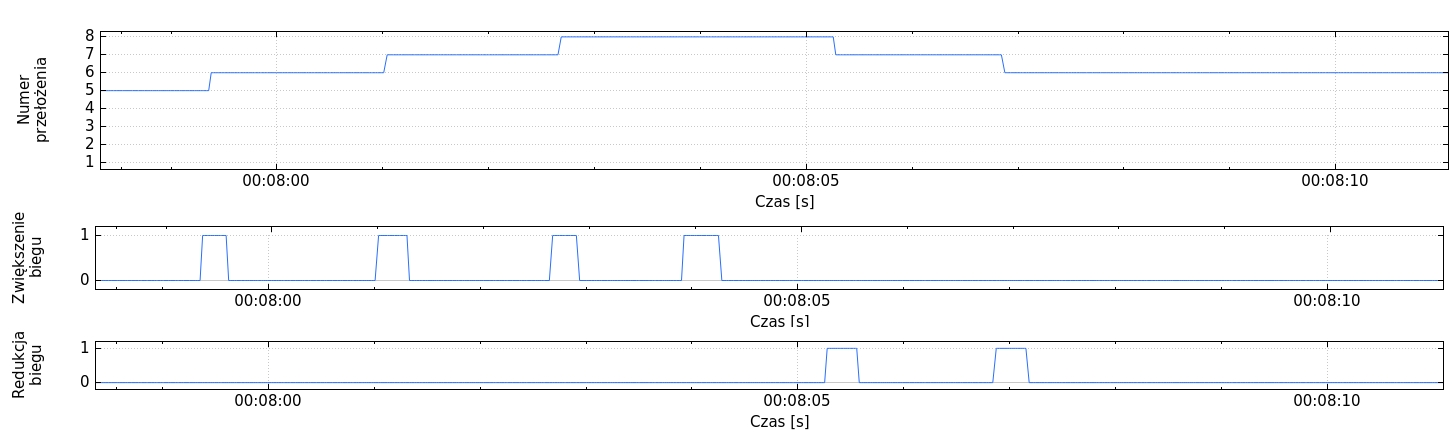
\includegraphics[scale=0.36]{tests_randomChange1.jpg}
    \caption{Zmiana przełożeń w trybie ręcznym}
    \label{fig:tests_randomChange}
\end{figure}

\begin{figure}[h]
    \centering
    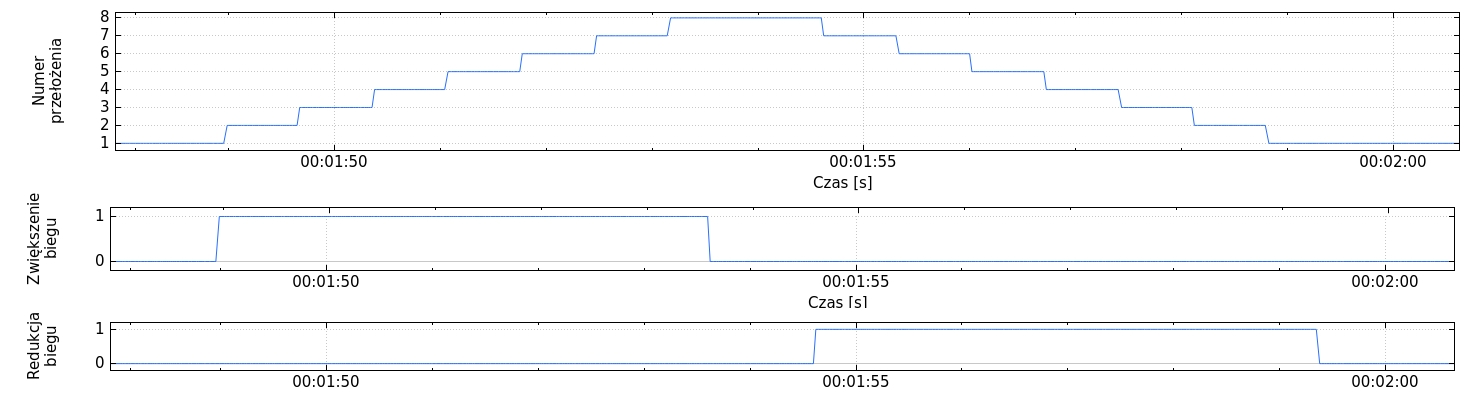
\includegraphics[scale=0.36]{tests_continousChange.jpg}
    \caption{Ciągła zmiana przełożeń}
    \label{fig:tests_continousChange}
\end{figure}
\subsection{Tryb comfort}

\subsection{Tryb active}

\subsection{Tryb sport}
